%!TeX encoding = UTF-8 Unicode
%!TeX spellcheck = en-UK
% !TeX root = Perrinet26mnesis.tex
% -*- coding: UTF-8; -*-
%%%-----------------------------------------------------------------
\begin{figure}%[htbp]
  \centering
  \adjustbox{valign=t,width=0.43\textwidth}{%
  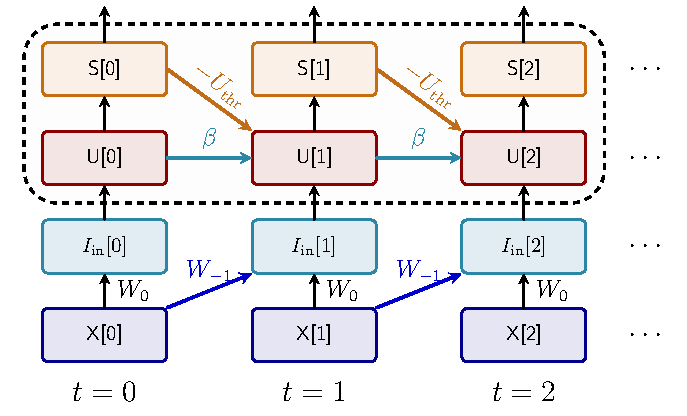
\includegraphics[width=\linewidth]{fig_snntorch.pdf}%
  }
    \hfill
    \adjustbox{valign=t}{
\includegraphics[width=0.52\textwidth]{pattern.pdf}}
  \caption{%
    Network architecture and a sample target pattern. \emph{Left:} Unrolled view of the recurrent HD-SNN over time (one column representing one time step), illustrating delayed connections between neurons: Blue arrows indicate synaptic connections that integrate past activity across heterogeneous delays; for clarity only one delay is shown. \emph{Right:} One representative target spike pattern ($N=1024$ neurons, $T=1000$ time steps, of which we show $256$ neurons and $400$ time steps); each red circle marks one target spike. The goal of the network is to memorise $M=16$ such patterns. Each trial is flanked by $N_\mathrm{pretime}=50$ time steps of spontaneous background activity (random spikes at rate $p_A$) before and after the stimulus. The trigger window (green crosses between the dashed lines) consists of the first $D=41$ time steps of the target pattern clamped to the network input; the recurrent network then autonomously predicts the remaining spikes.
  }\label{fig:model}
\end{figure}
%%%-----------------------------------------------------------------
